\documentclass[11pt]{beamer}
%\usetheme{Madrid}
\usetheme{Warsaw}
\setbeamercovered{transparent}
\useoutertheme{infolines}


\usefonttheme{serif}

\usepackage{tikz}
\usetikzlibrary{arrows.meta}
\usepackage[utf8]{inputenc}
\usepackage[T1]{fontenc}
\usepackage{amsmath}
\usepackage{amsfonts}
\usepackage{amssymb}
\usepackage{graphicx}
\usepackage{bookmark}
\usepackage{caption}
\DeclareMathOperator{\sen}{sen}
\DeclareMathOperator{\tg}{tg}
\setbeamertemplate{caption}[numbered]

%%%%%%%%%%%%%% MISE EN PAGE DE LA PREMIERE SLIDE %%%%%%%%%%%%%%
\author[Matis Viozelange]{Matis Viozelange}
\title{Model Following Control Applied to a Three Dimensional Overhead Crane}
\newcommand{\email}{matis.viozelange@eleves.ec-nantes.fr}
\setbeamertemplate{navigation symbols}{} % Remove navigation symbols
\logo{
  \hfill
\includegraphics[scale=0.04]{imgs/TU_Ilmenau_Logo_black_green.svg.png}%
  \hfill
\includegraphics[scale=0.08]{imgs/LogoCN_Q.pdf}%
}
\institute[]{Ecole Centrale de Nantes \\ Technische Universität Ilmenau}
\date{\today}

%%%%%%%%%%%%%% Custom footline %%%%%%%%%%%%%%
\setbeamertemplate{footline}{
  \leavevmode%
  \hbox{%
    \begin{beamercolorbox}[wd=.333333\paperwidth,ht=2.25ex,dp=1ex,center]{author in head/foot}%
      \usebeamerfont{author in head/foot}\insertshortauthor
    \end{beamercolorbox}%
    \begin{beamercolorbox}[wd=.333333\paperwidth,ht=2.25ex,dp=1ex,center]{title in head/foot}%
      \usebeamerfont{title in head/foot}\hspace*{2em}
      Model Following Control
      \hspace*{2em}
    \end{beamercolorbox}%
    \begin{beamercolorbox}[wd=.333333\paperwidth,ht=2.25ex,dp=1ex,right]{date in head/foot}%
      \usebeamerfont{date in head/foot}\insertshortdate \hspace*{4em} \insertframenumber{} / \inserttotalframenumber\hspace*{2ex}
    \end{beamercolorbox}%
  }%
  \vskip0pt%
}

%%%%%%%%%%%%%% Subsection Content Recall %%%%%%%%%%%%%%
\AtBeginSubsection[
  {\frame<beamer>{\frametitle{Outline}   
    \tableofcontents[currentsection,currentsubsection]}}%
]%
{
  \frame<beamer>{ 
    \frametitle{Outline}   
    \tableofcontents[currentsection,currentsubsection]}
}

\begin{document}

\begin{frame}
\titlepage
\end{frame}

\begin{frame}{Table of Contents}
\tableofcontents
\end{frame}


\section{Introduction}

\subsection{Crane presentation and control goals}

\begin{frame}{The crane System}
\framesubtitle{Real Crane}
\begin{figure}
    \centering
    \rotatebox{270}{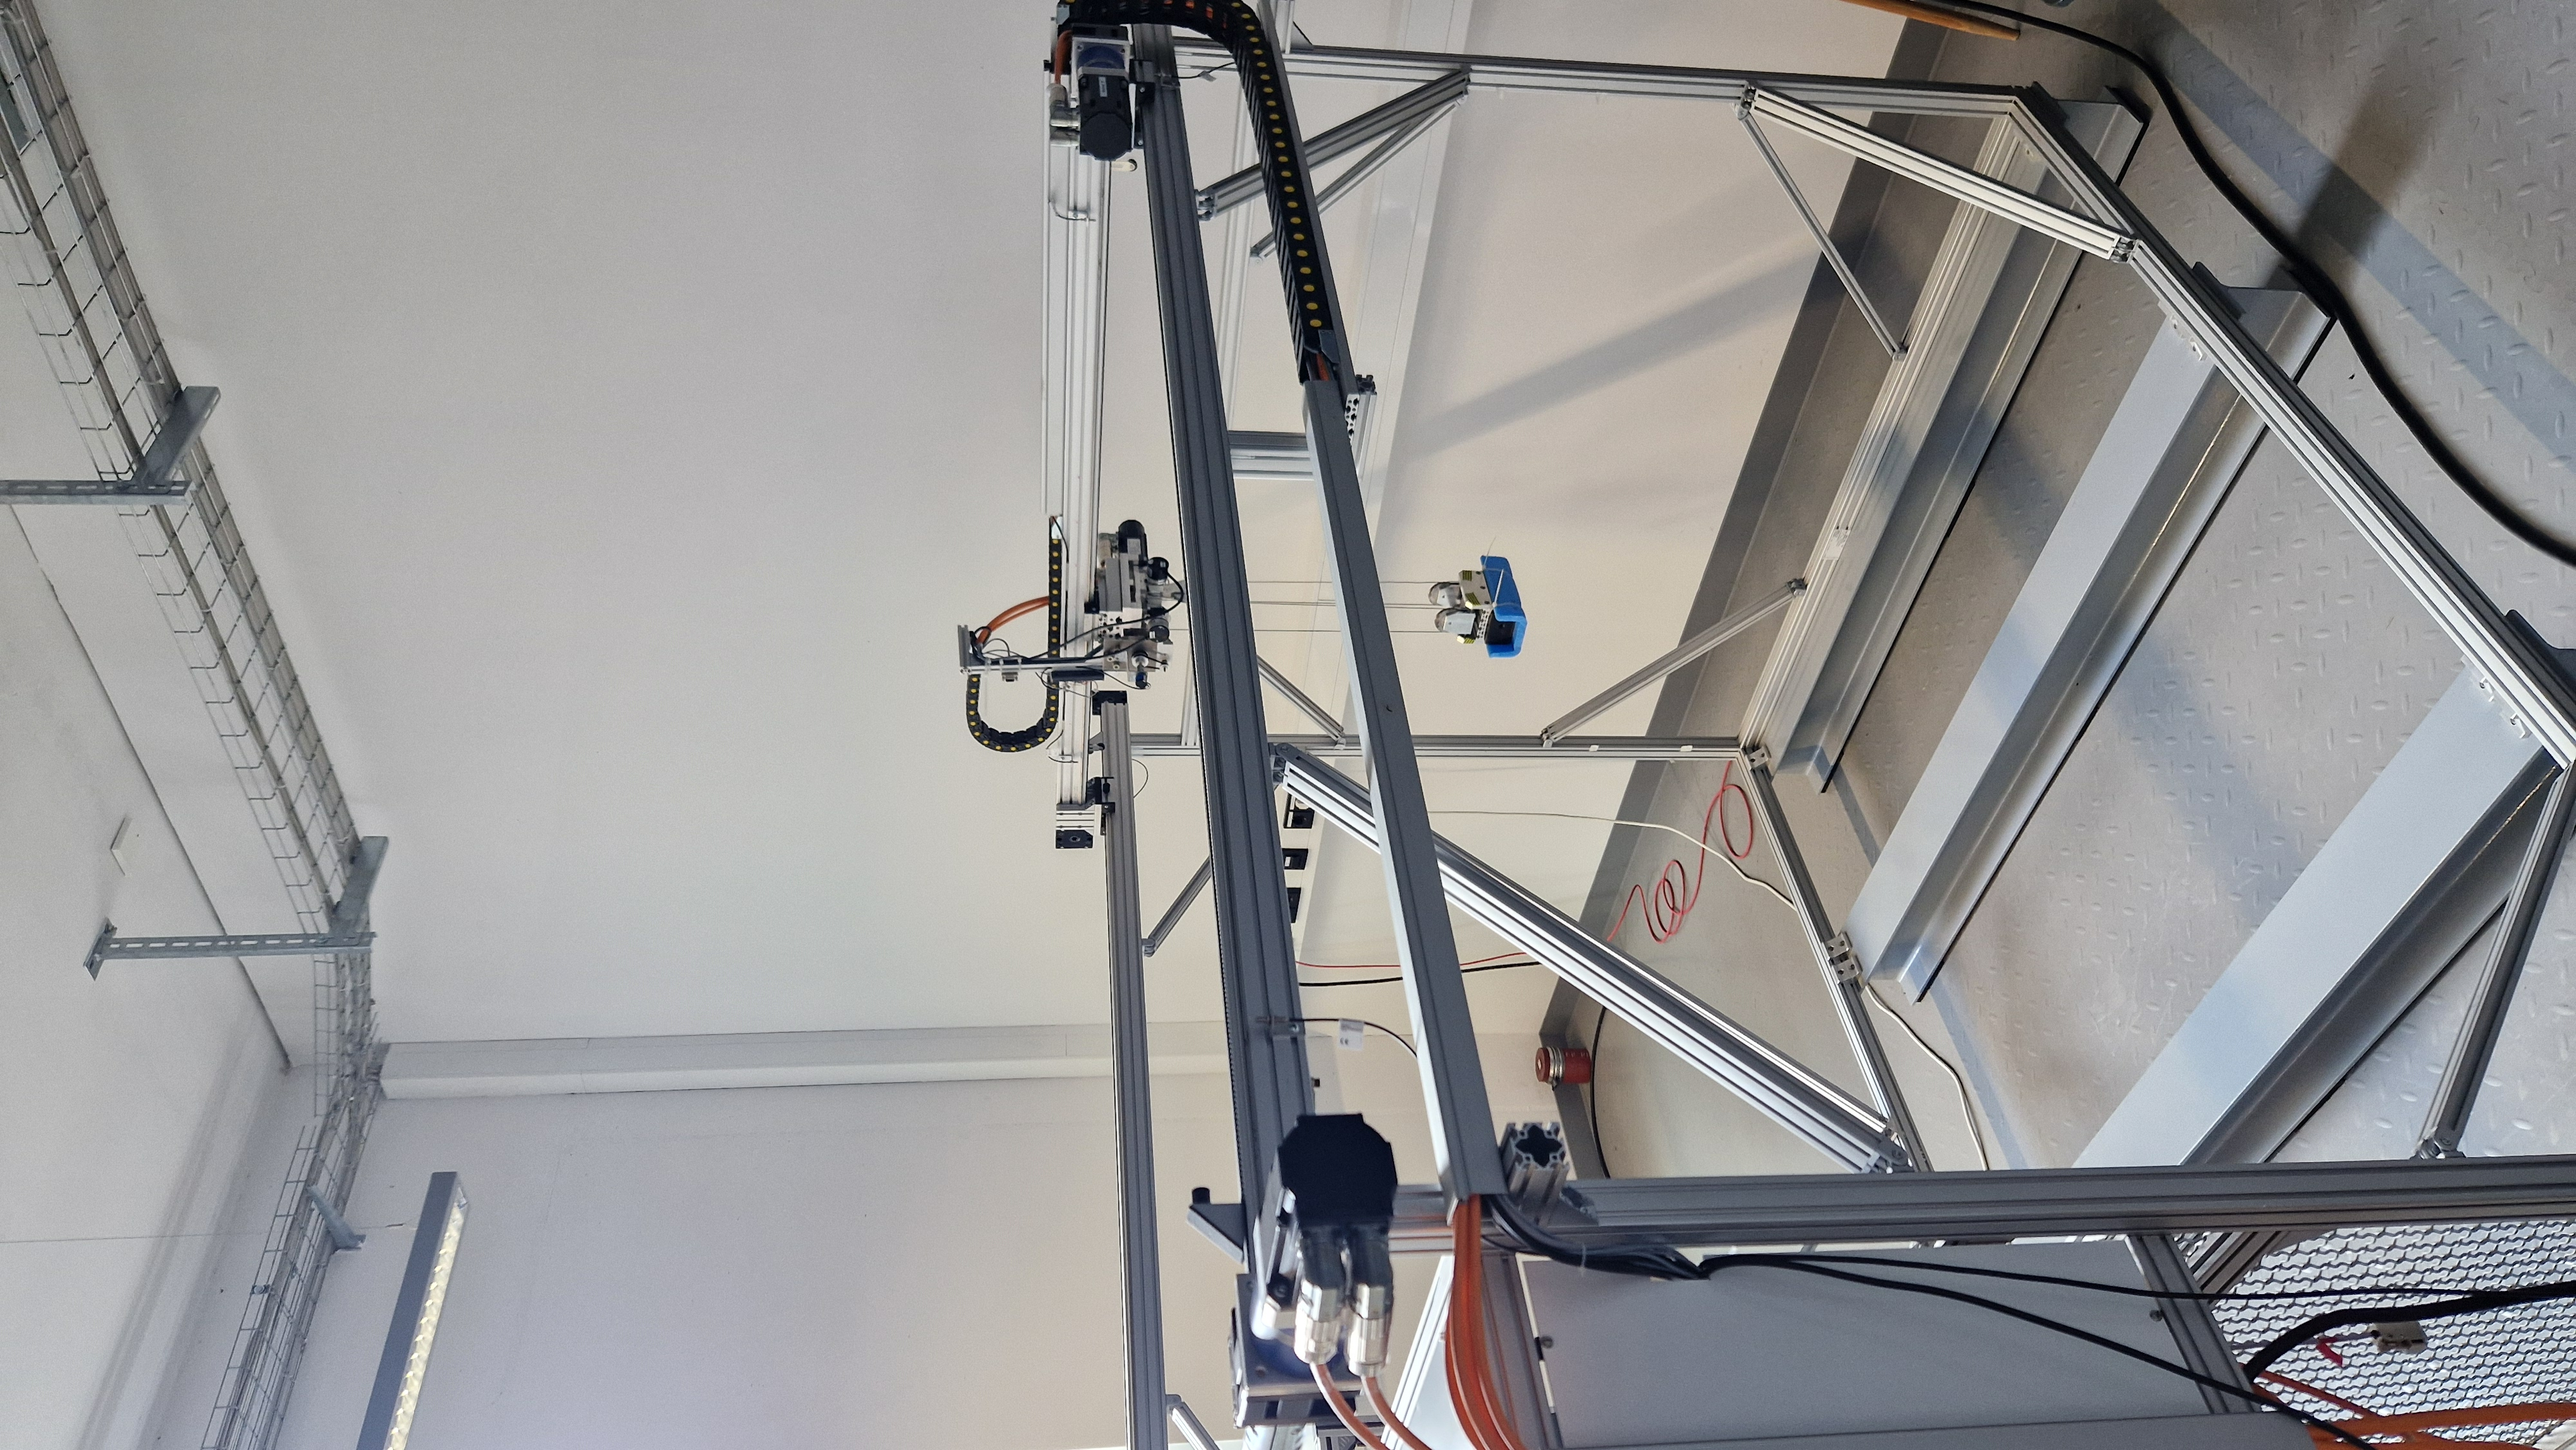
\includegraphics[width=0.5\linewidth]{imgs/Simulation/General.jpg}}
    \caption{Real 3-dim overhead Crane}
\end{figure}
\end{frame}



\begin{frame}{The crane System}
\framesubtitle{Scheme}
    \begin{figure}
        \centering
        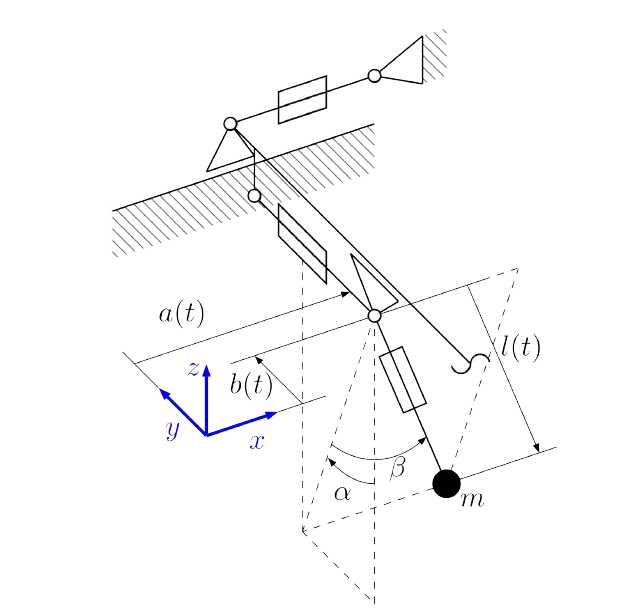
\includegraphics[width=0.5\linewidth]{imgs/Crane/3DimCranSchem.PNG}
        \caption{Schematics of three dimensional overhead crane \cite{Knierim2010Crane}}
        \label{fig:Schematics of three dimensional overhead crane}
    \end{figure}
\end{frame}

\begin{frame}{Control Goals}
     The goals of this work are : 
    \begin{itemize}
        \item Implement a Model Following Control (MFC) to make the crane's load track set points and trajectories 
        \item Highlight the attenuation of the peaking phenomenon by the MFC
    \end{itemize}

\end{frame}


%______________________________________________________________________________%
\section{Crane Overview}
\subsection{Crane Model}
\begin{frame}{The Trolley}
\begin{columns}[T]
    \begin{column}{0.5\textwidth}
        \centering
        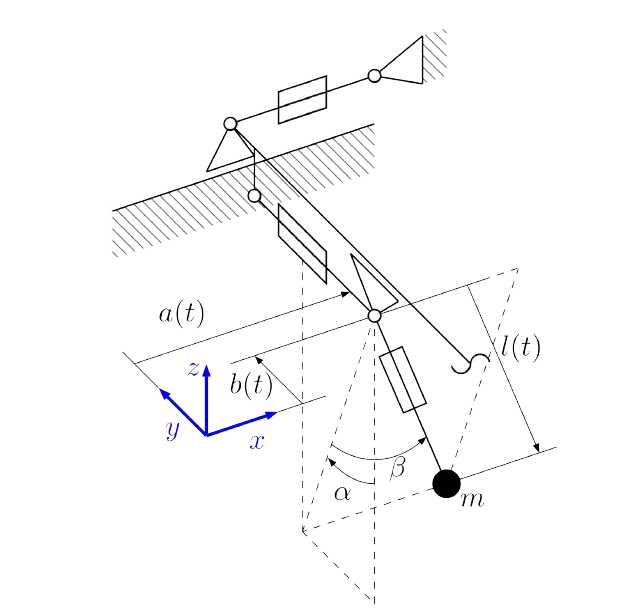
\includegraphics[width=\linewidth]{imgs/Crane/3DimCranSchem.PNG}
        \captionof{figure}{Schematics of three dimensional overhead crane \cite{Knierim2010Crane}}
        \label{fig:Schematics of three dimensional overhead crane}
    \end{column}
    \begin{column}{0.5\textwidth}
        First, the crane dynamic equations are computed as in \cite{Knierim2010Crane}. The trolley position \(\boldsymbol{r}_{t}(t)\) is considered as a time-dependent function given by:

         \vspace{1em} % Add vertical space
         
        \begin{equation}
            \textbf{r}_t(t) = \begin{bmatrix}
                a(t) & b(t) & 0
            \end{bmatrix}^T
        \end{equation}

         \vspace{1em} % Add vertical space
         
        where \(a(t)\) and \(b(t)\) are the positions of the trolley in the \(x\) and \(y\) directions.
    \end{column}
\end{columns}
\end{frame}


\begin{frame}{System output}
\begin{columns}[T]
\begin{column}{0.5\textwidth}
        \centering
        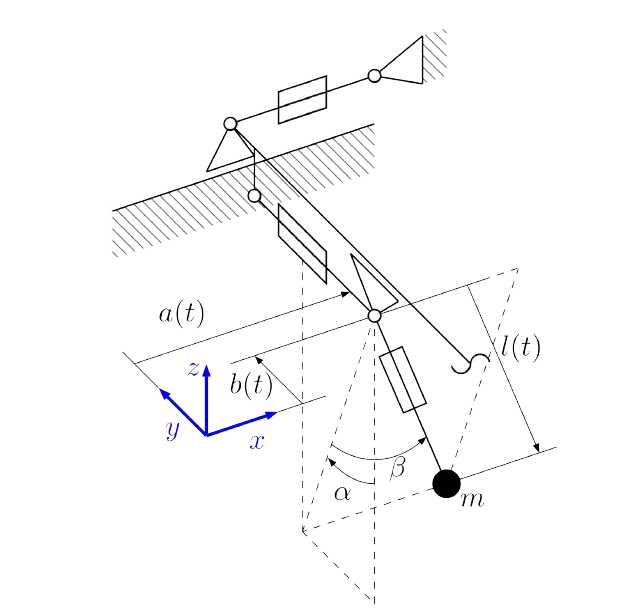
\includegraphics[width=\linewidth]{imgs/Crane/3DimCranSchem.PNG}
        \captionof{figure}{Schematics of three dimensional overhead crane \cite{Knierim2010Crane}}
        \label{fig:Schematics of three dimensional overhead crane}
\end{column}
    
\begin{column}{0.5\textwidth}
    The position of the load, which will be the output of the system as \(\textbf{y}(t)\) given by :

 \vspace{1em} % Add vertical space
 
\begin{equation}
    \textbf{y}(t) = \begin{bmatrix}
        a(t) + l(t)S_\beta \\
    b(t) + l(t)C_\beta S_\alpha \\
    -l(t)C_\beta C_\alpha
    \end{bmatrix}
\end{equation}

 \vspace{1em} % Add vertical space
 

With the notations \(S_\gamma = sin(\gamma)\) and \(C_\gamma = cos(\gamma)\).
\end{column}

\end{columns}

\end{frame}

\begin{frame}{Dynamic Equation}
 We define the generalized coordinates vector \(\boldsymbol{\theta} = \left[ \alpha \; \beta \right]^T\) to get the Newton-Euler equation of the load system. 

 First let's note  \( \boldsymbol{J}_{l}(t)\), the jacobian of the crane over the generalized coordinates : 

\begin{equation}
     \boldsymbol{J}_{l}(t) = \frac{\partial \boldsymbol{y}(t)}{\partial \boldsymbol{\theta}} = \begin{bmatrix}
         0                       & l(t)C_\beta \\
         l(t)C_\beta C_\alpha    & -l(t)S_\beta S_\alpha \\
         l(t)C_\beta S_\alpha    & l(t)S_\beta C_\alpha
     \end{bmatrix}
\end{equation}
\end{frame}

\begin{frame}{Dynamic Equation}
The velocity and acceleration of the load are given by : 
\begin{align}
    \dot{\boldsymbol{y}} &= \boldsymbol{J}_{l}(t) \dot{\theta} + \underbrace{ \left. \frac{\partial \boldsymbol{y}}{\partial t} \right\|_{\theta=cst}}_{\bar{\dot{\boldsymbol{y}}}(t)} \\
    \ddot{\boldsymbol{y}} &= \boldsymbol{J}_{l}(t) \ddot{\theta} + \underbrace{\frac{d\boldsymbol{J}_{l}(t)}{dt} \cdot \dot{\boldsymbol{\theta}} + \frac{d\bar{\dot{\boldsymbol{y}}}(t)}{dt}}_{\bar{\ddot{\boldsymbol{y}}}(t)}
\end{align}
\end{frame}

\begin{frame}{Crane Model Overview}
    After some steps and by applying the Newton-Euler equation, the system reads :
    \begin{equation}
\label{eq:equation_of_motion_generalized_coordinates}
    \boldsymbol{J}_{l}(t)^T\boldsymbol{J}_{l}(t)\cdot \ddot{\boldsymbol{\theta}} = -\boldsymbol{J}_{l}(t)^T \: \bar{\ddot{\boldsymbol{y}}}(t) \; + \; \boldsymbol{J}_{l}(t)^T\boldsymbol{g}
\end{equation}

Where \(\boldsymbol{g} = \begin{bmatrix} 0 & 0 & -g\end{bmatrix}^T\) denotes the gravity vector.
\end{frame}

\begin{frame}{Dynamic Equation}
 The input is be the same as in the simulation and the real crane experimentation, they will directly drive the \(\begin{bmatrix}\ddot{a}(t) & \ddot{b}(t) & \ddot{l}(t)\end{bmatrix}\) coordinates. Which gives us the complete dynamics of the crane plant system in the form of a non-linear vectorial second order differential equation \cite{Knierim2010Crane} : 


\begin{align}
\left\{ \begin{array}{ll}
\ddot{a}(t) &= u_1\\ 
\ddot{b}(t) &= u_2\\ 
\ddot{l}(t) &= u_3\\
\ddot{\alpha}(t) &= \frac{1}{l(t) C_{\beta}} \left(2 \dot{\alpha} \dot{\beta} S_{\beta} l(t) - 2 \dot{l}(t) \dot{\alpha} C_{\beta} - S_{\alpha} g - C_{\alpha} u_2\right) \\
\ddot{\beta}(t) &= \frac{1}{l(t)} \left(-C_{\alpha} S_{\beta} g - S_{\beta} C_{\beta} \dot{\alpha}^2 l(t) - 2 \dot{l}(t) \dot{\beta} + S_{\beta} S_{\alpha} u_2 - C_{\beta} u_1\right) \\
\end{array}
\right.
\end{align}

and the output :  \(\textbf{y}(t) \)

\end{frame}

\begin{frame}{Dynamic Equation}
 We can now write this system into the normal form : 

\begin{align*}
    \dot{\boldsymbol{x}} &= \boldsymbol{f}(\boldsymbol{x}) + \boldsymbol{g}(\boldsymbol{x})\boldsymbol{u} \\
     \boldsymbol{y}  &= \boldsymbol{h}(\boldsymbol{x})
\end{align*}

where : 
\begin{align*}
    \boldsymbol{x}(t) &= (x_i(t))_{1\le i\le 10} \\ &= \begin{pmatrix} a(t) & \dot{a}(t) & b(t) & \dot{b}(t) & l(t) & \dot{l}(t) & \alpha(t) & \dot{\alpha}(t) & \beta(t) & \dot{\beta}(t)\end{pmatrix}^T
\end{align*}
Denotes the state vector

It is required for a system to be in Byrnes-Isidori to apply MFC. Exact feedback linearization is used in this MIMO system.
\end{frame}
%_______________________________________________________________________%

\subsection{Feedback linearization and dynamic extension}

\begin{frame}{Dynamic Extension}

The Feedback linearization applied directly to the crane equation has internal dynamics. One solution is to artificially increase the relative degree of \(y_3\) by implementing a dynamic extension as in \cite{Noack2020} by introducing a virtual control input that reads : 
\begin{align}
    \ddot{\nu} &= w_3 \\
    u_3 &= \psi(\boldsymbol{x}, \nu)
\end{align}

\(u_3\) is computed so that \(
    \forall t \ge 0 \; , \quad \ddot{y}_3(t) - \nu(t) = 0\) 
\end{frame}



\begin{frame}{Feedback Linearization}
   \begin{itemize}
       \item  With our crane system, the relative degrees of our outputs \([y_1, y_2, y_3]^T\) are respectively \([2, 2, 2]^T\), which leads to internal dynamics. 

       \item One way to address this issue is to artificially increase the relative degree of \(y_3\) by applying the previous dynamical extension that has in our case the propriety ti increase the relative degrees to  \([4, 4, 4]^T\).
   \end{itemize}
\end{frame}


\begin{frame}{Feedback Linearization}
    Now it can be shown that by applying the following transformation to each output \(y_i\) for \(i \in \{1, 2, 3\}\) of the system,

\begin{equation}
\boldsymbol{\xi}_i
=
\boldsymbol{T}_i(\boldsymbol{x})
=
\begin{bmatrix}
    y_i \\
    \dot{y}_i \\
    \ddot{y}_i \\
    y^{(3)}_i
\end{bmatrix}
\end{equation}

The system is divided into 3 decoupled subsystems in Byrnes-Isidori form that read : 

\begin{equation}
\label{eq:flat_sys_reduced}
\forall i \in \{1, 2, 3\} : 
\left\{
\begin{aligned}
  \dot{\boldsymbol{\xi}_i} &= \boldsymbol{A} \boldsymbol{\xi}_i + \boldsymbol{B} \big(a_i(\boldsymbol{\xi}) + b_i(\boldsymbol{\xi})u)\\
  \boldsymbol{y}_i &= \boldsymbol{C} \boldsymbol{\xi}_i 
\end{aligned}
\right.
\end{equation}
\end{frame}




\section{Model Following Control}

\subsection{Overview}
%_______________________________________________________________________%
\begin{frame}{Control Loop}
    \begin{figure}[htb]
        \caption{Model Following control block diagram with model control loop process and control loop \cite{Willkomm2023MFC}}
        \label{fig:MFC Control Loop}
        \centering
        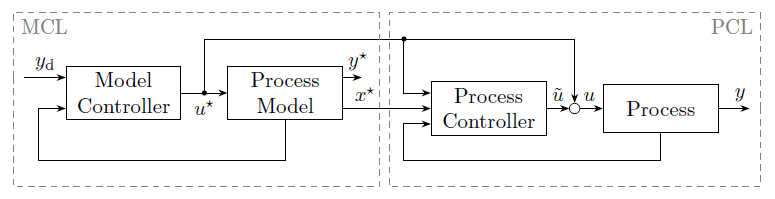
\includegraphics[width=0.8\textwidth]{imgs/MFC/MFC_scheme.PNG}
        \end{figure}
\end{frame}

%_______________________________________________________________________%
\begin{frame}{General Equation}
Consider the flat system : 
\begin{equation}
\label{eq:flat_sys_reduced}
\left\{
\begin{aligned}
  \dot{\xi} &= A\xi + B\big(a(\xi) + b(\xi)u + \Delta(\xi, t) \big) \\
  y &= C\xi
\end{aligned}
\right.
\end{equation}



where  and \( \xi(t) \in \mathbb{D}_\xi \subseteq \mathbb{R}^n \) denote the states. 
\(\Delta: \mathbb{D}_{\xi} \times \mathbb{R}^+ \rightarrow \mathbb{R}\) are the perturbations. \\
The output is \( y(t) \in \mathbb{R} \) and \( u(t) \in \mathbb{R} \) denotes the input. The relative degree is \( n \ge 1 \). 

 \begin{block}{Remark}
    Here we consider a SISO system. That doesn't matter as the crane's 3 outputs are decoupled. The control loop can be separated into 3 distinct SISO control loops of dimension 4.
    \end{block}

\end{frame}

\begin{frame}{General Equation}
The matrices \( A \), \( B \), and \( C \) are given by:

\begin{align*}
A &=
\begin{bmatrix}
0 & 1 & 0 & \cdots & 0 \\
0 & 0 & 1 & \cdots & 0 \\
\vdots & \vdots & \ddots & \ddots & \vdots \\
0 & 0 & \cdots & 0 & 1 \\
0 & 0 & \cdots & 0 & 0
\end{bmatrix}
\in \mathbb{R}^{n \times n}, \quad
B =
\begin{bmatrix}
0 \\
0 \\
\vdots \\
0 \\
1
\end{bmatrix}
\in \mathbb{R}^n, \\
C &=
\begin{bmatrix}
1 & 0 & \cdots & 0
\end{bmatrix}
\in \mathbb{R}^{1 \times n}
\end{align*}
\end{frame}


%_______________________________________________________________________%
\subsection{Model Control Loop (MCL)}
\begin{frame}{MCL Dynamics}
    An analysis of the control loop dynamics can be carried out in two stages. First, we consider the Model Control Loop (MCL), which is a replica of system \ref{eq:flat_sys_reduced}, excluding the perturbations \(\Delta\), and is described by:

\begin{equation}
\label{eq:MCL_open_loop}
  \dot{\xi^*} = A\xi^* + B\big(a(\xi^*) + b(\xi^*)u^* \big)
\end{equation}

\end{frame}

\begin{frame}{Open Loop dynamics}
    We write :  \(u = \tilde{u} + u^*\), where \(u^*\) : the output of the MCL and \(\tilde{u}\) : the output of the process control loop \\
    The error states are defined as \(\tilde{\xi} = \xi - \xi^*\), and the open-loop dynamics of the MFC are given by:

\begin{align}
\dot{\xi}^* &= A\xi^* + B \left( a(\xi^*) + b(\xi^*) u^* \right) \\
\dot{\tilde{\xi}} &= A\tilde{\xi} + B \left( \tilde{a}(\xi^*, \tilde{\xi}, u^*) + b(\xi^* + \tilde{\xi}) \tilde{u} + \Delta(\xi^* + \tilde{\xi}, t)  \right)
\end{align}

where

\begin{align}
\tilde{a}(\xi^*, \tilde{\xi}, u^*) &= a(\xi^* + \tilde{\xi}) - a(\xi^*) + \left( b(\xi^* + \tilde{\xi}) - b(\xi^*) \right) u^*
\end{align}


\end{frame}


\begin{frame}{Feedback Linearization}
    
Ensure closed-loop stability : a feedback linearization law is applied to the MCL  defined by:

\begin{equation}
\label{eq:MCL_control_law}
u^* = -\frac{a(\xi^*) + v^*}{b(\xi^*)}
\end{equation}

The design of \(v^*\) is based on the error dynamics within the MCL : \(\tilde{\xi}^* = \xi^* - \xi_d\) representing the deviation between the model and desired states. The associated error dynamics are given by:

\begin{align}
\dot{\tilde{\xi}}^* &= A\tilde{\xi}^* + B(v^* - y_d^{(r)})
\end{align}

\end{frame}



\begin{frame}{Closed Loop Dynamics}
The new input \(v^*\) is chosen as:

\begin{equation}
v^* = y_d^{(r)} + K\tilde{\xi}^*
\end{equation}

where \(K = [-\alpha_0, -\alpha_1, \ldots, -\alpha_{r-1}] \in \mathbb{R}^{1 \times r}\) is selected such that the matrix \(A + BK\) is Hurwitz. The closed-loop dynamics of the MCL become:

\begin{align}
\dot{\tilde{\xi}}^* &= (A + BK)\tilde{\xi}^*
\end{align}
\end{frame}


%_______________________________________________________________________%

\subsection{Process Control Loop (PCL)}
\begin{frame}{Introduction}
    The process control loop is design to counter the perturbations and model uncertainties. The design method to assure robustness is the high-control gain approach. The desired output trajectory \(y_d(t) \in \mathbb{R}\) is assumed to be at least n-times continuously differentiable. The desired external states \(\xi_d(t) \in \mathbb{D}_{\xi_d}  \subseteq \mathbb{R}^n\) are generated by 

\begin{equation}
    \dot{\xi_d} = A\xi_d + By_d^{(n)}
\end{equation}

\end{frame}

\begin{frame}{Open Loop Dynamics}
    The open-loop error dynamics :

\begin{align}
\dot{\tilde{\xi}} &= A\tilde{\xi} + B\left(\tilde{a}(\xi^*, \tilde{\xi}, u^*) + b(\tilde{\xi}^* + \tilde{\xi}) \tilde{u} + \Delta(\tilde{\xi}^* + \tilde{\xi}, t) \right)
\end{align}

The design of the process controller will also be a feedback linearizing control law :

\begin{equation}
\tilde{u} = \frac{-\tilde{a}(\xi^*, \tilde{\xi}, u^*) + \tilde{K}\tilde{\xi}}{b(\xi^* + \xi)}
\end{equation}

where : \(\tilde{K} = KD^{-1}\varepsilon^{-1}\) with \(D = \text{diag}(\varepsilon^{n}, \varepsilon^{n-1}, \ldots, 1)\) and \(0 < \varepsilon < 1\) is a time scaling parameter.

\end{frame}

\begin{frame}{Overall Dynamics}
    
We proceed the time scaling change of variable : 

\begin{equation}
    \zeta = D^{-1}\tilde{\xi}
\end{equation}

The closed-loop overall dynamics of the MFC scheme for set-point and trajectory tracking are given by

\begin{align}
\label{eq:The closed-loop overall dynamics of the MFC}
\dot{\tilde{\xi}}^* &= (A + BK)\tilde{\xi}^* \\
\varepsilon\dot{\zeta} &= (A + BK)\zeta + \varepsilon B \left(\Delta(\xi_d + \tilde{\xi}^* + D\zeta, t) \right).
\end{align}

\end{frame}

\begin{frame}{Process Control Loop}
    \begin{itemize}
    \item If \( A + BK \) is Hurwitz, the eigenvalues of the error dynamics (without time-scaling) can be shifted arbitrarily far to the left of the imaginary axis as \( \epsilon \rightarrow 0 \).
    \item Theoretically, the error dynamics can be made to converge arbitrarily quickly.
    \item Achieving this may necessitate a significantly large control effort.
    \item A small \( \epsilon \) enhances robustness against perturbations \( \Delta(\xi, t) \). One can with this assumption : 
    \[
    |\Delta(\xi, t)| \leq \delta + L_\Delta \lVert \xi \rVert_2
    \]
    Find a condition on \(\epsilon\) to encounter the perturbations.
    \item Additionally, a small \( \epsilon \) accelerates the error dynamics of the PCL.
\end{itemize}
\end{frame}



%_______________________________________________________________________%
\begin{frame}{A Simpler Design}
\cite{Tietze2023CruiseControl} showed a simpler architecture of the MFC, which includes the following key points:

\begin{itemize}
    \item The feedback linearization control law is given by:
    \(
    u = \frac{-a(\xi) + y_d^{(n)} + v}{b(\xi)}
    \)
    where \( v = v^* + \tilde{v} \).

    \item The dynamics of the open loop are described by:
    \[
    \dot{\xi} = A\xi + B(y_d^{(n)} + v) + \Delta(\xi, t)
    \]

    \item The nominal model of the external dynamics is given by the integrator chain:
    \[
    \dot{\xi}^* = A\xi^* + B(y_d^{(n_\xi)} + v^*)
    \]
    with the initial state \(\xi^*(0) = \xi_0^*\), and the error dynamics:
    \[
    \dot{\tilde{\xi}} = A\tilde{\xi} + B(\tilde{v} + \Delta(\xi, \eta, t))
    \]
\end{itemize}
\end{frame}

\begin{frame}{A Simpler Design}
\cite{Tietze2023CruiseControl} continued:

\begin{itemize}
    \item The dynamics of the open-loop MFC system include:
 \begin{align}
    \dot{\tilde{\xi}}^* &= A\tilde{\xi}^* + Bv^* \\
    \dot{\tilde{\xi}} &= A\tilde{\xi} + B(\tilde{v} + \Delta(\xi, t))
 \end{align}
    
    \item One can rewrite the control loop as follows : 

    \begin{figure}
        \centering
        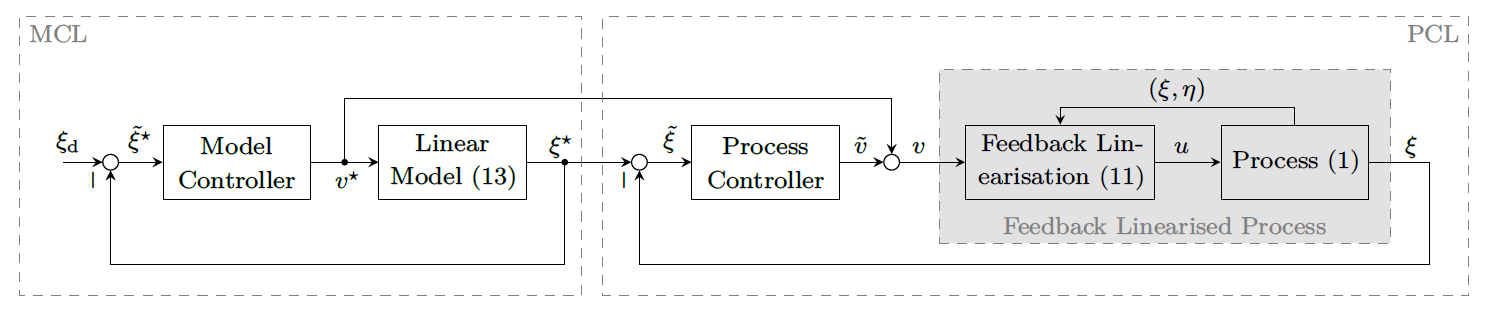
\includegraphics[width=0.9\linewidth]{imgs/MFC/MFCEfficient.PNG}
        \caption{Block-diagram of the MFC architecture with linear model of the feedback linearized process \cite{Tietze2023CruiseControl}}
        \label{fig:Blockdiagram of the MFC architecture with linear model of the feedback linearised process}
    \end{figure}

\end{itemize}
\end{frame}

\begin{frame}{Control Loops Comparison}
    \begin{figure}
        \centering
        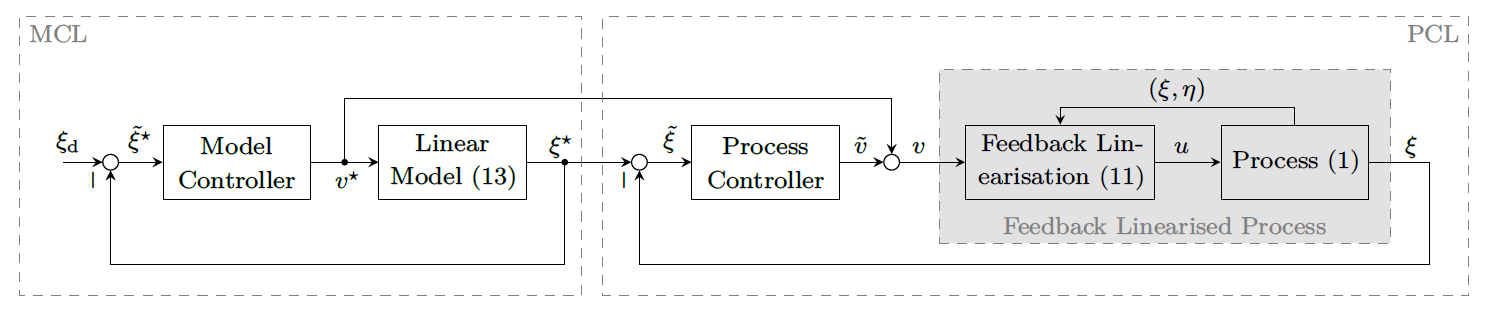
\includegraphics[width=0.9\linewidth]{imgs/MFC/MFCEfficient.PNG}
        
        \label{fig:Blockdiagram of the MFC architecture with linear model of the feedback linearised process}
    \end{figure}

     \begin{figure}
       
        \label{fig:MFC Control Loop}
        \centering
        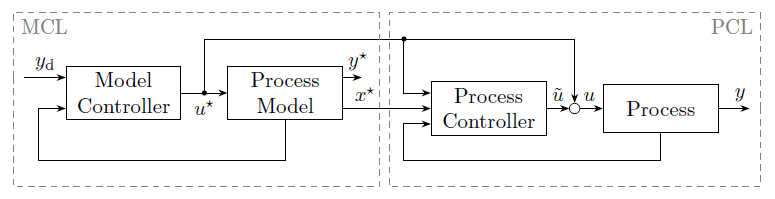
\includegraphics[width=0.9\textwidth]{imgs/MFC/MFC_scheme.PNG}
     \end{figure}

    
\end{frame}


%_______________________________________________________________________%

\subsection{High Gain Control Comparison}
\begin{frame}{High Gain Control}

The High Gain Control law is formulated as:

\begin{equation}
u = \frac{-a(\xi) + K_\epsilon \xi }{b(\xi)}
\end{equation}

\begin{itemize}
    \item With only one loop in the control. The slower motion of the MCL are not present and the PCL alone try to stabilize the dynamics.

    \item This control law is designed to aggressively reduce the error, leading to rapid convergence to the desired state.
\end{itemize}

\end{frame}


\begin{frame}{Peaking Phenomenon}
    
However, it is clear that we have peaking with this method, which is characterized by:

\begin{block}{Peaking Phenomenon}
Peaking refers to large transient peaks in control signals or state variables, caused by high gain amplifying initial errors or disturbances. This can lead to:
\begin{itemize}
    \item Large temporary deviations in system response.
    \item Potential saturation of actuators, resulting in performance degradation or instability.
    \item Challenges in systems with fast dynamics or constrained states.
\end{itemize}
\end{block}

\end{frame}



\section{Results}
\subsection{Simulation Results}
%_______________________________________________________________________%
\begin{frame}{Implementation on Matlab}
    \begin{figure}
        \centering
        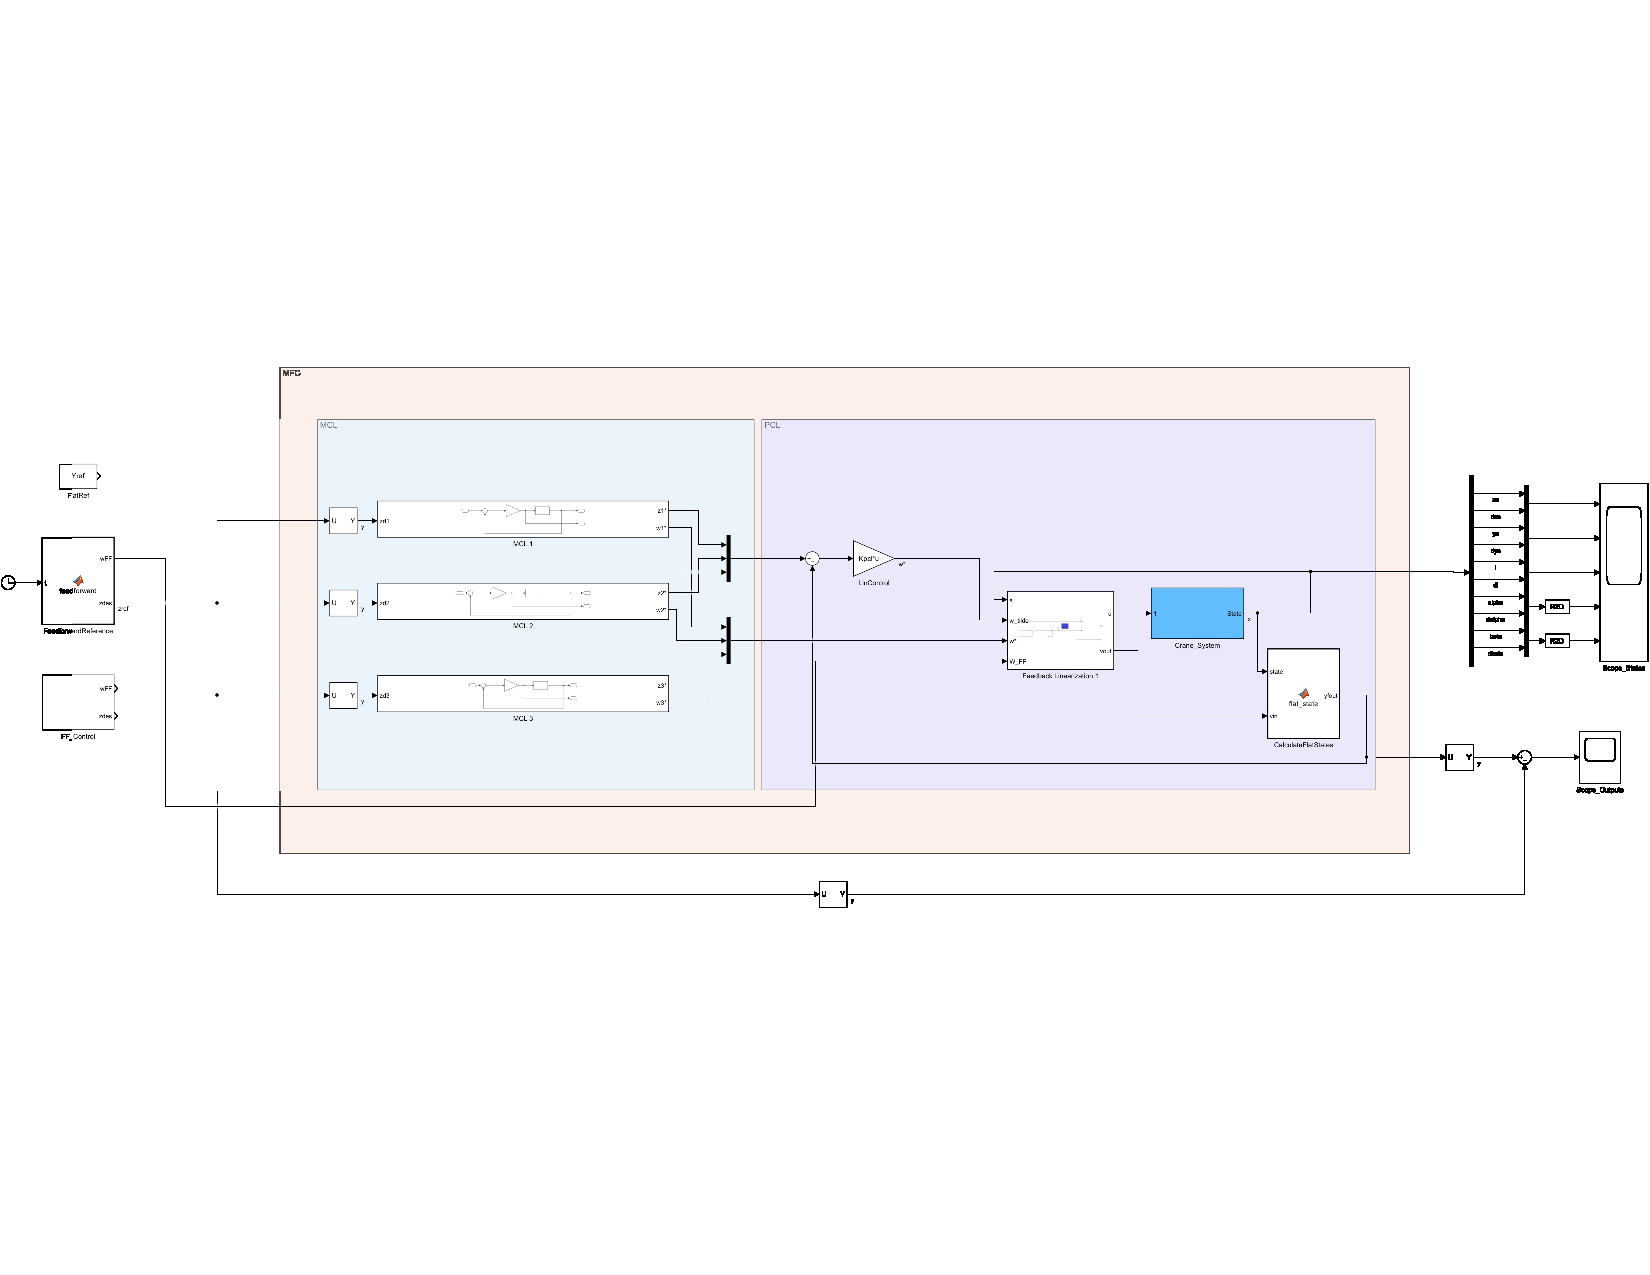
\includegraphics[width=0.9\linewidth]{imgs/Simulation/MFC_efficient_model.pdf}
        \caption{Simulink Model MFC Loop}
        \label{fig:Simulink Model MFC Loop}
    \end{figure}
\end{frame}


%_______________________________________________________________________%
\begin{frame}{Set‐Point Tracking in the Experiment}
    Here is the desired trajectory : 
    \begin{figure}
        \centering
        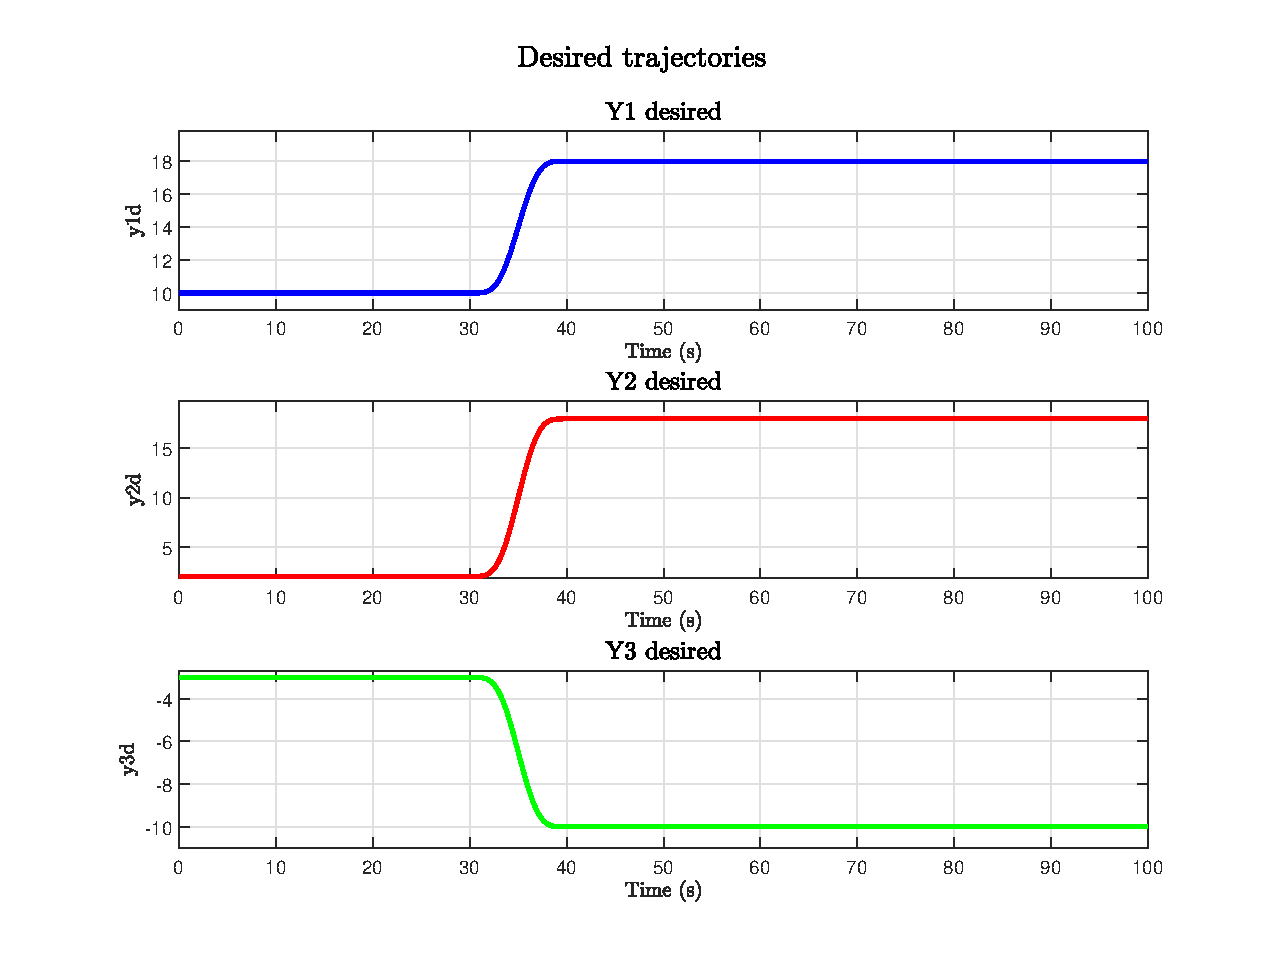
\includegraphics[width=0.75\linewidth]{imgs/Simulation/desiredTraj.eps}
        \caption{Desired Trajectories of the Load}
    \end{figure}
\end{frame}


\begin{frame}{Simulation Results}
\begin{figure}
    \centering
    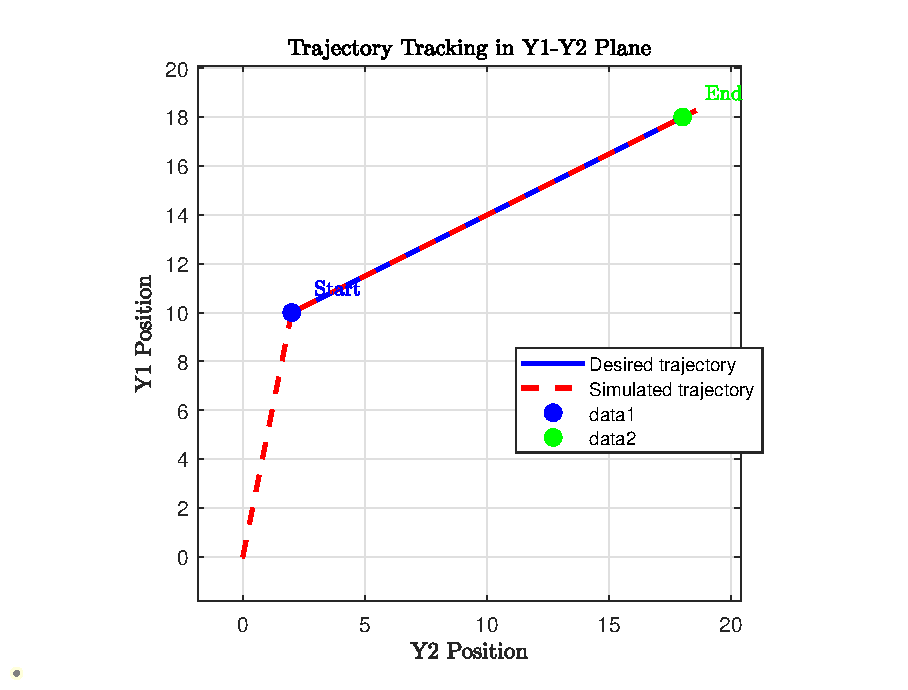
\includegraphics[width=0.8\linewidth]{imgs/Simulation/XYTrajectory.eps}
    \caption{Difference between CI desired states and Model States}
\end{figure}

\end{frame}



\begin{frame}{Simulation Results}
\framesubtitle{High Gain}
    \begin{figure}
    \centering
    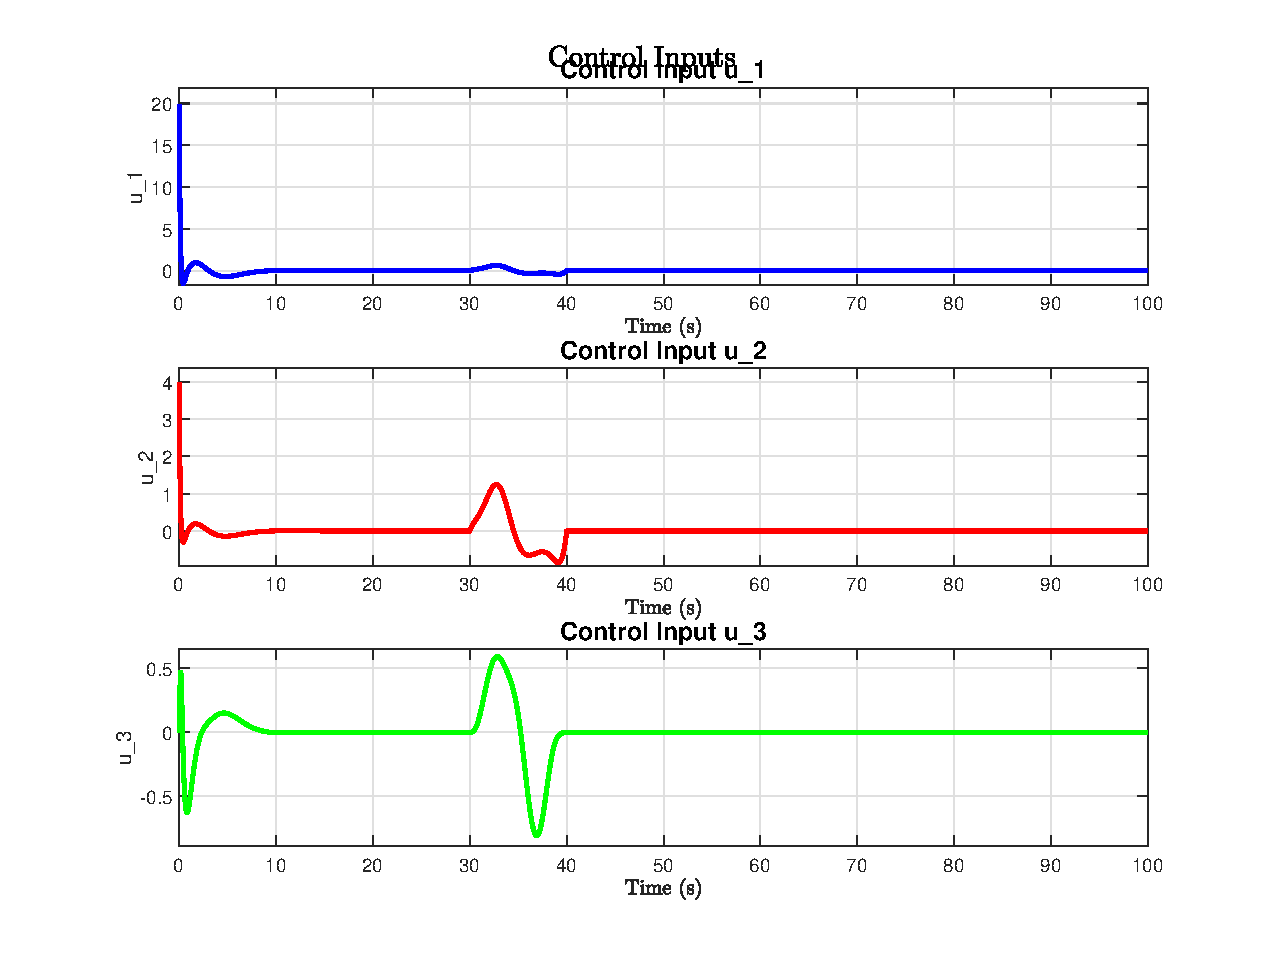
\includegraphics[width=0.8\linewidth]{imgs/Simulation/u_HG.eps}
    \caption{Input for Set point tracking High gain control}
\end{figure}
\end{frame}


\begin{frame}{Simulation Results}
\framesubtitle{MFC}
    \begin{figure}
        \centering
        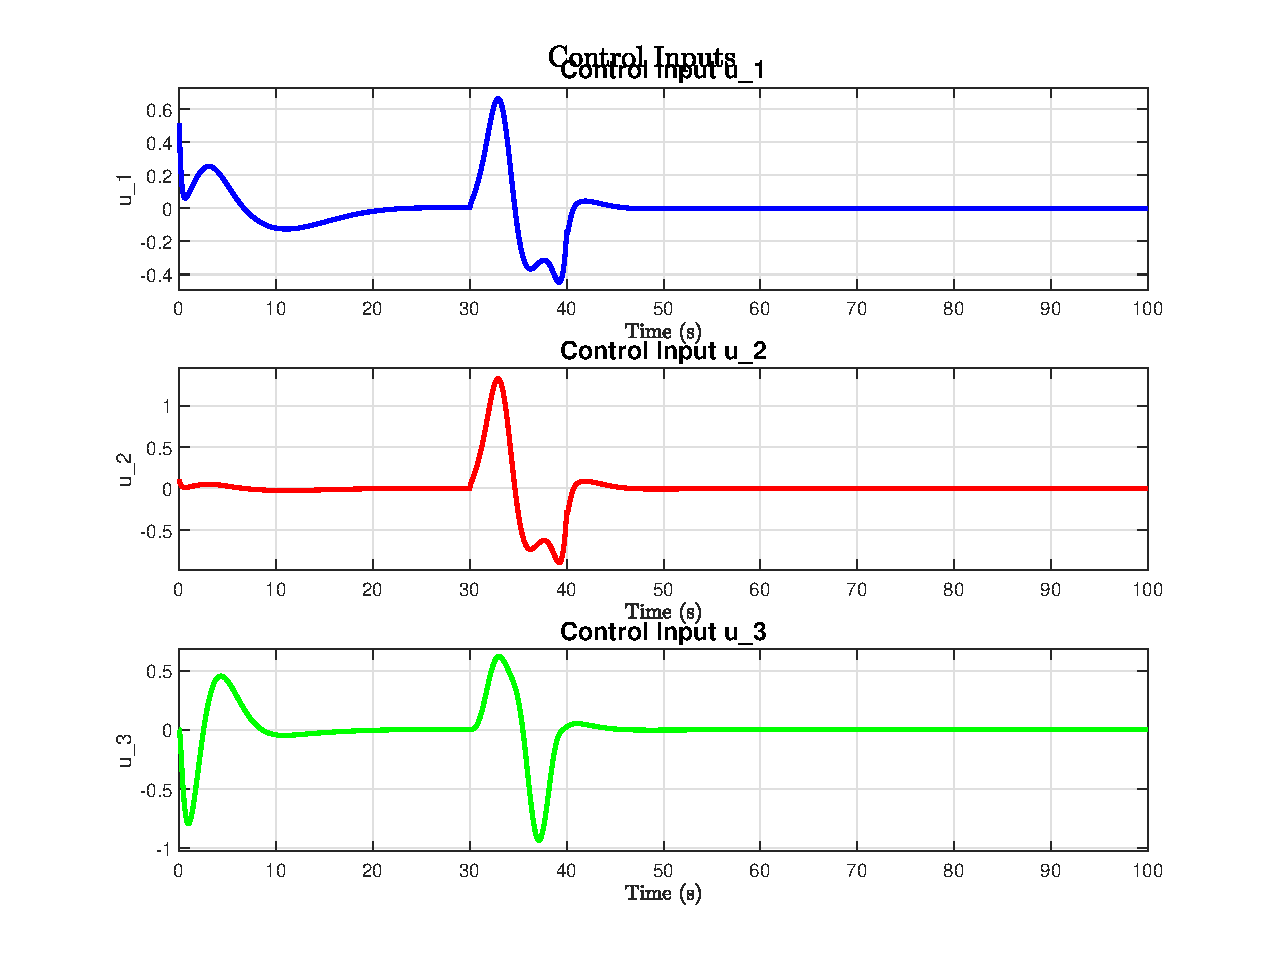
\includegraphics[width=0.8\linewidth]{imgs/Simulation/u_efficientMFC_Good_CI.eps}
        \caption{Input for Set point tracking MFC}
        \label{fig:input-mfc}
    \end{figure}
\end{frame}




    







%_______________________________________________________________________%
\subsection{Real Plant Experiment}
\begin{frame}{Presentation}
\framesubtitle{The Trolley and the Load}

\begin{figure}
    \centering
    \rotatebox{270}{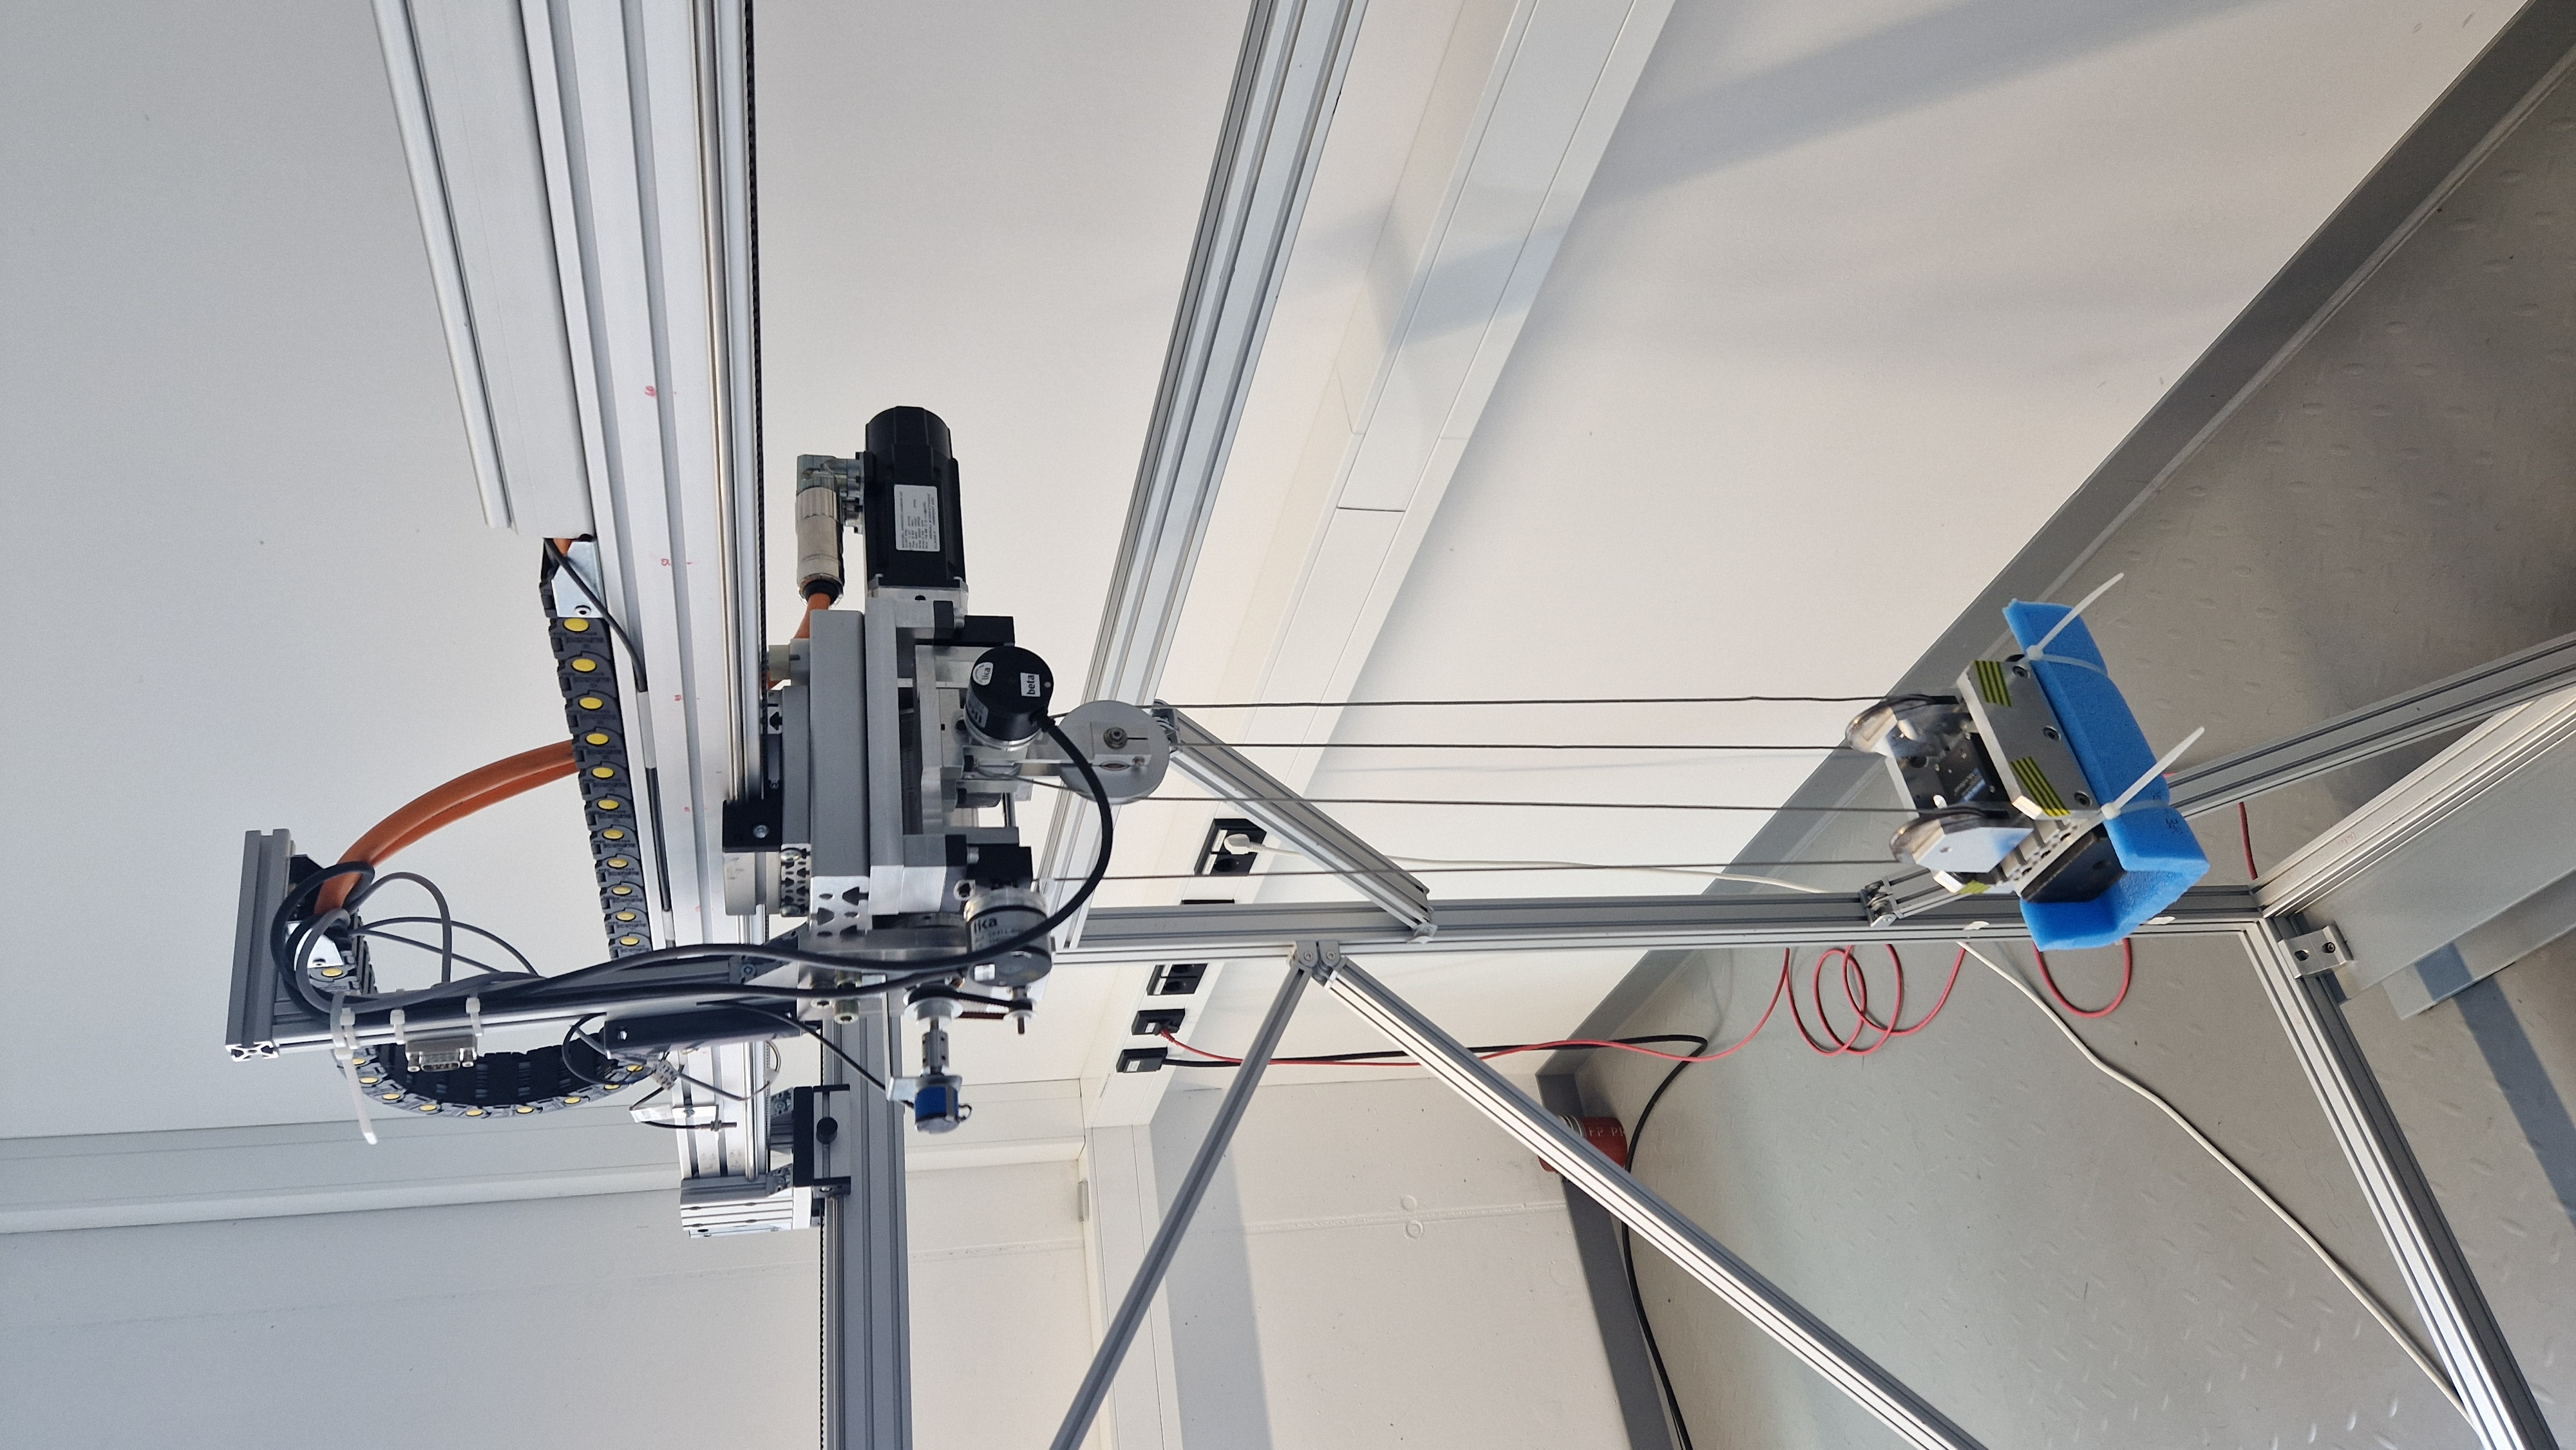
\includegraphics[width=0.5\linewidth]{imgs/Simulation/Trolley.jpg}}
    \caption{Zoom on the crane's trolley}
\end{figure}
\end{frame} 

\begin{frame}{X and Y motors}
\begin{columns}[T] % [T] aligns the columns at the top
    \begin{column}{0.5\textwidth} % Specify width for the first column
        \centering
        \rotatebox{270}{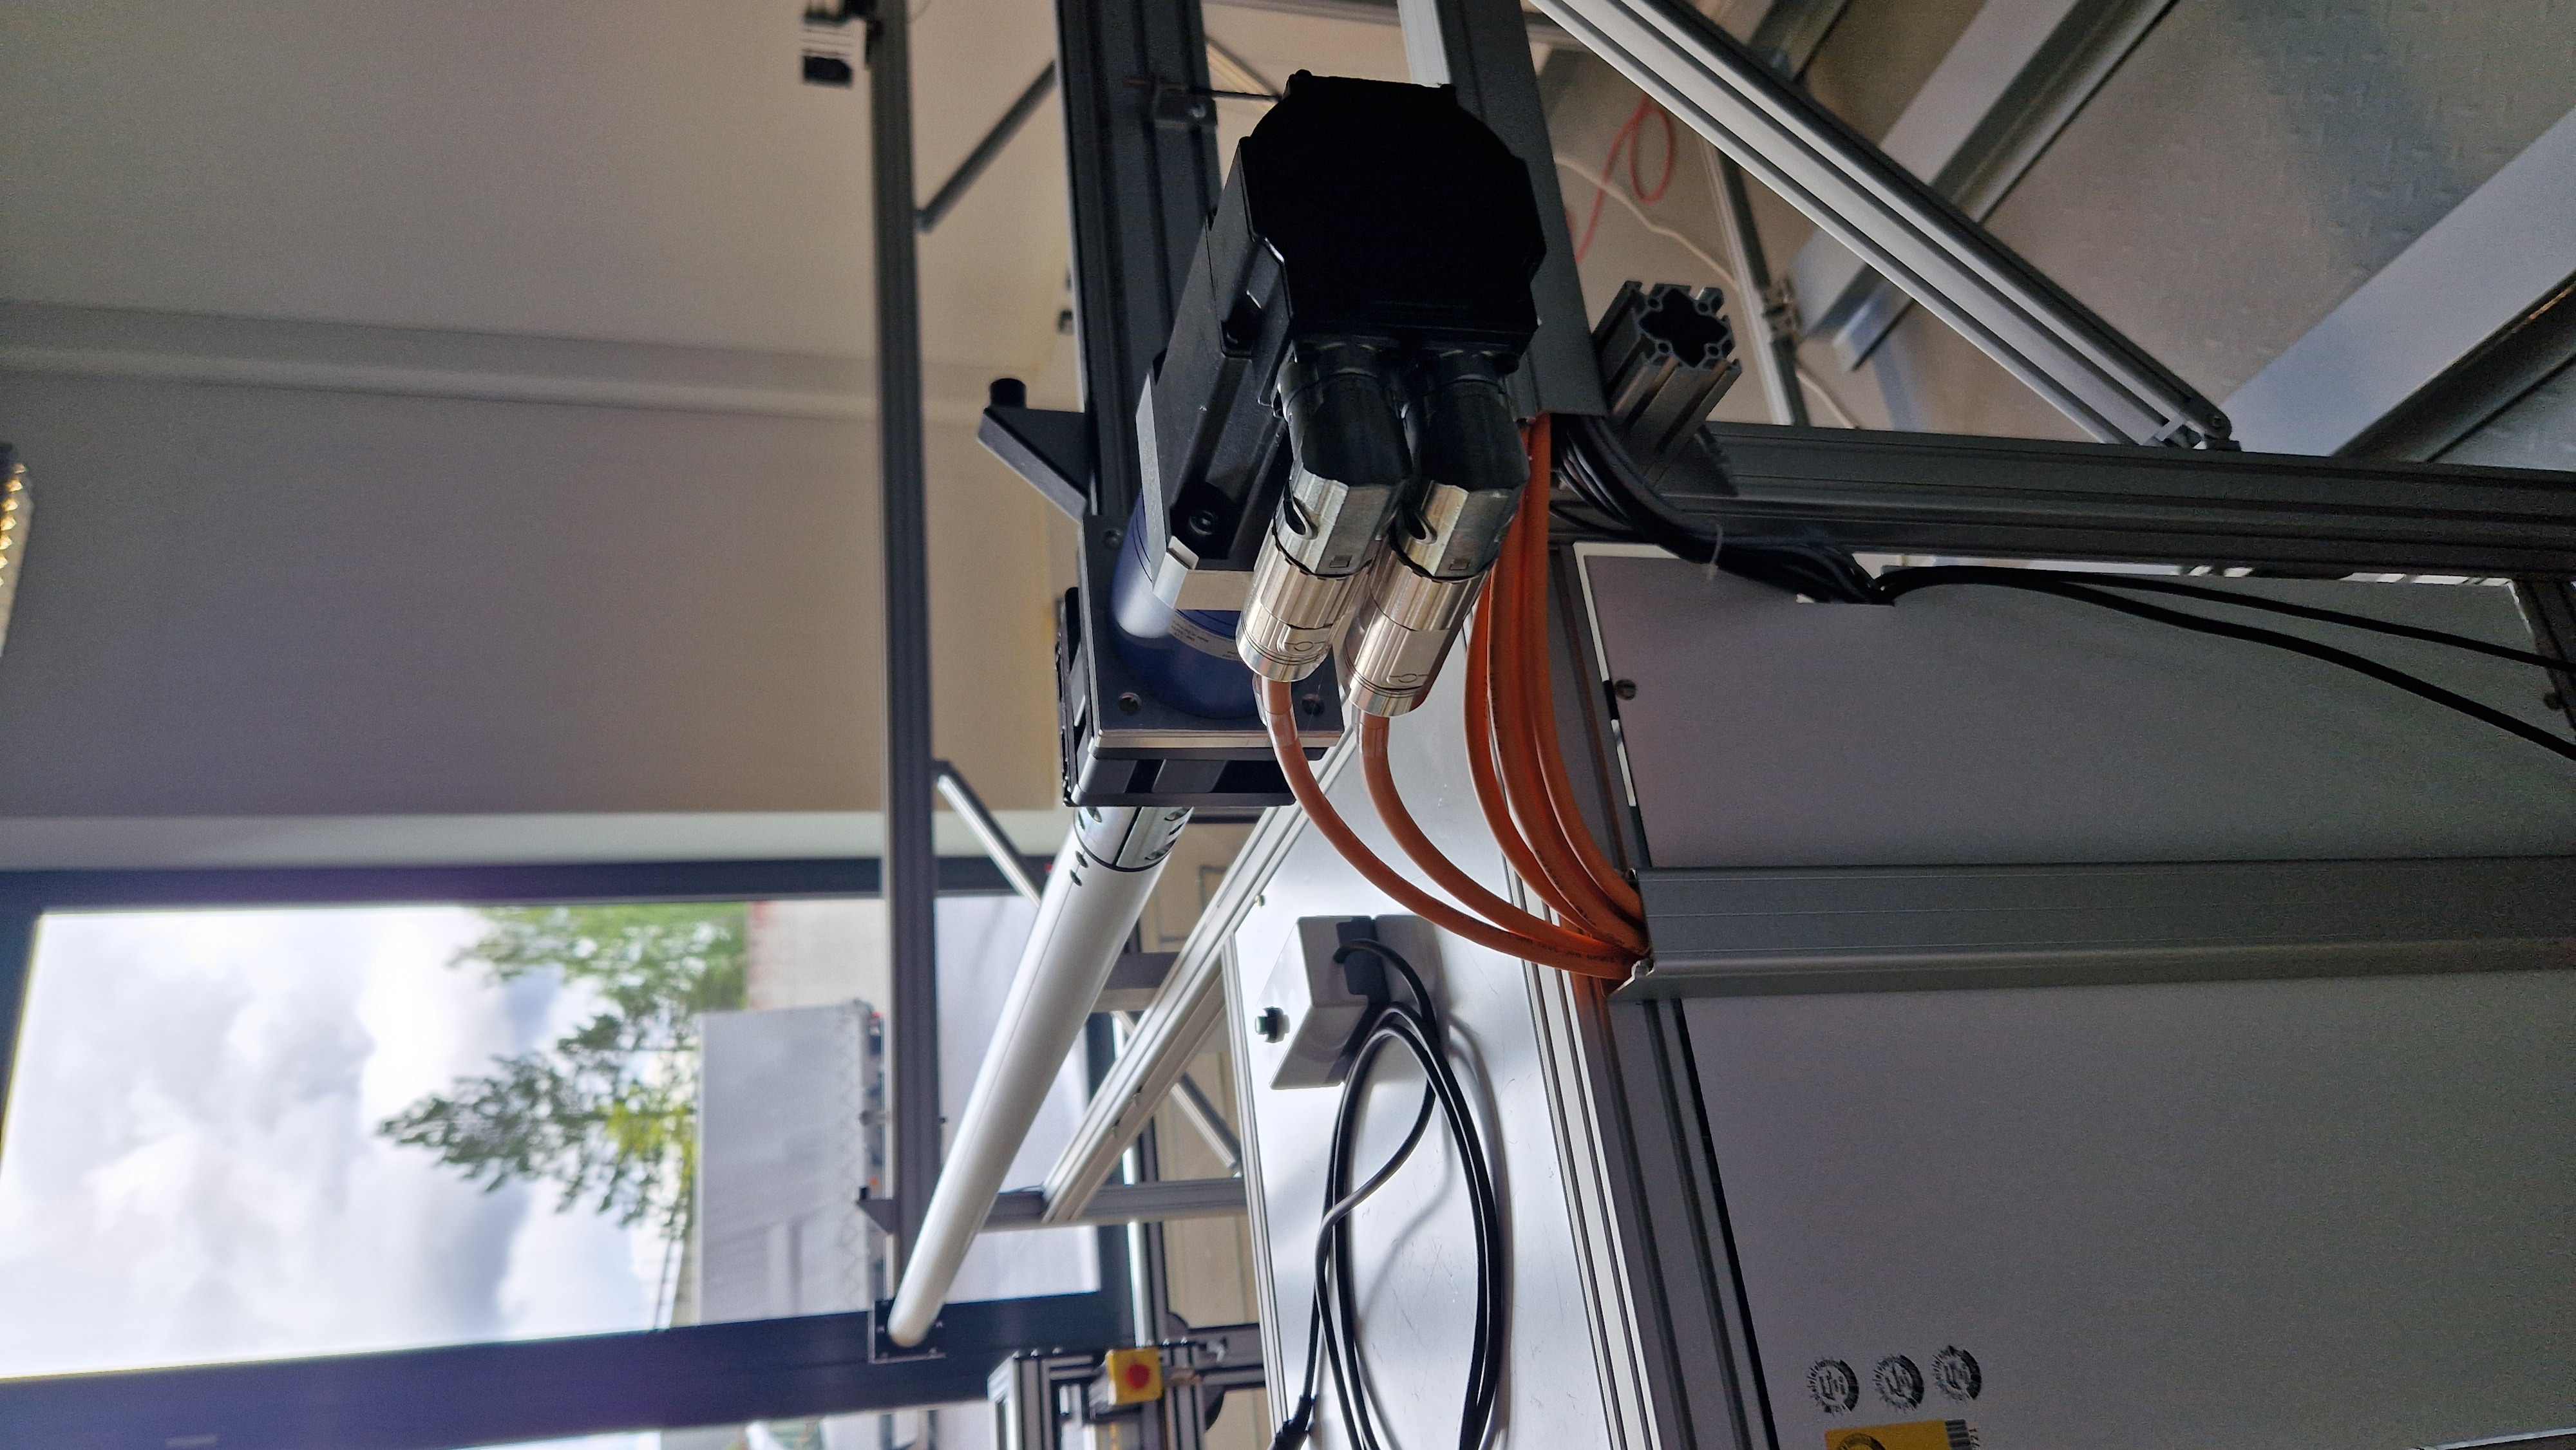
\includegraphics[width=\linewidth]{imgs/Simulation/Xmot.jpg}}
        \captionof{figure}{Zoom on X motor}
    \end{column}
    \begin{column}{0.5\textwidth} % Specify width for the second column
        \centering
        \rotatebox{270}{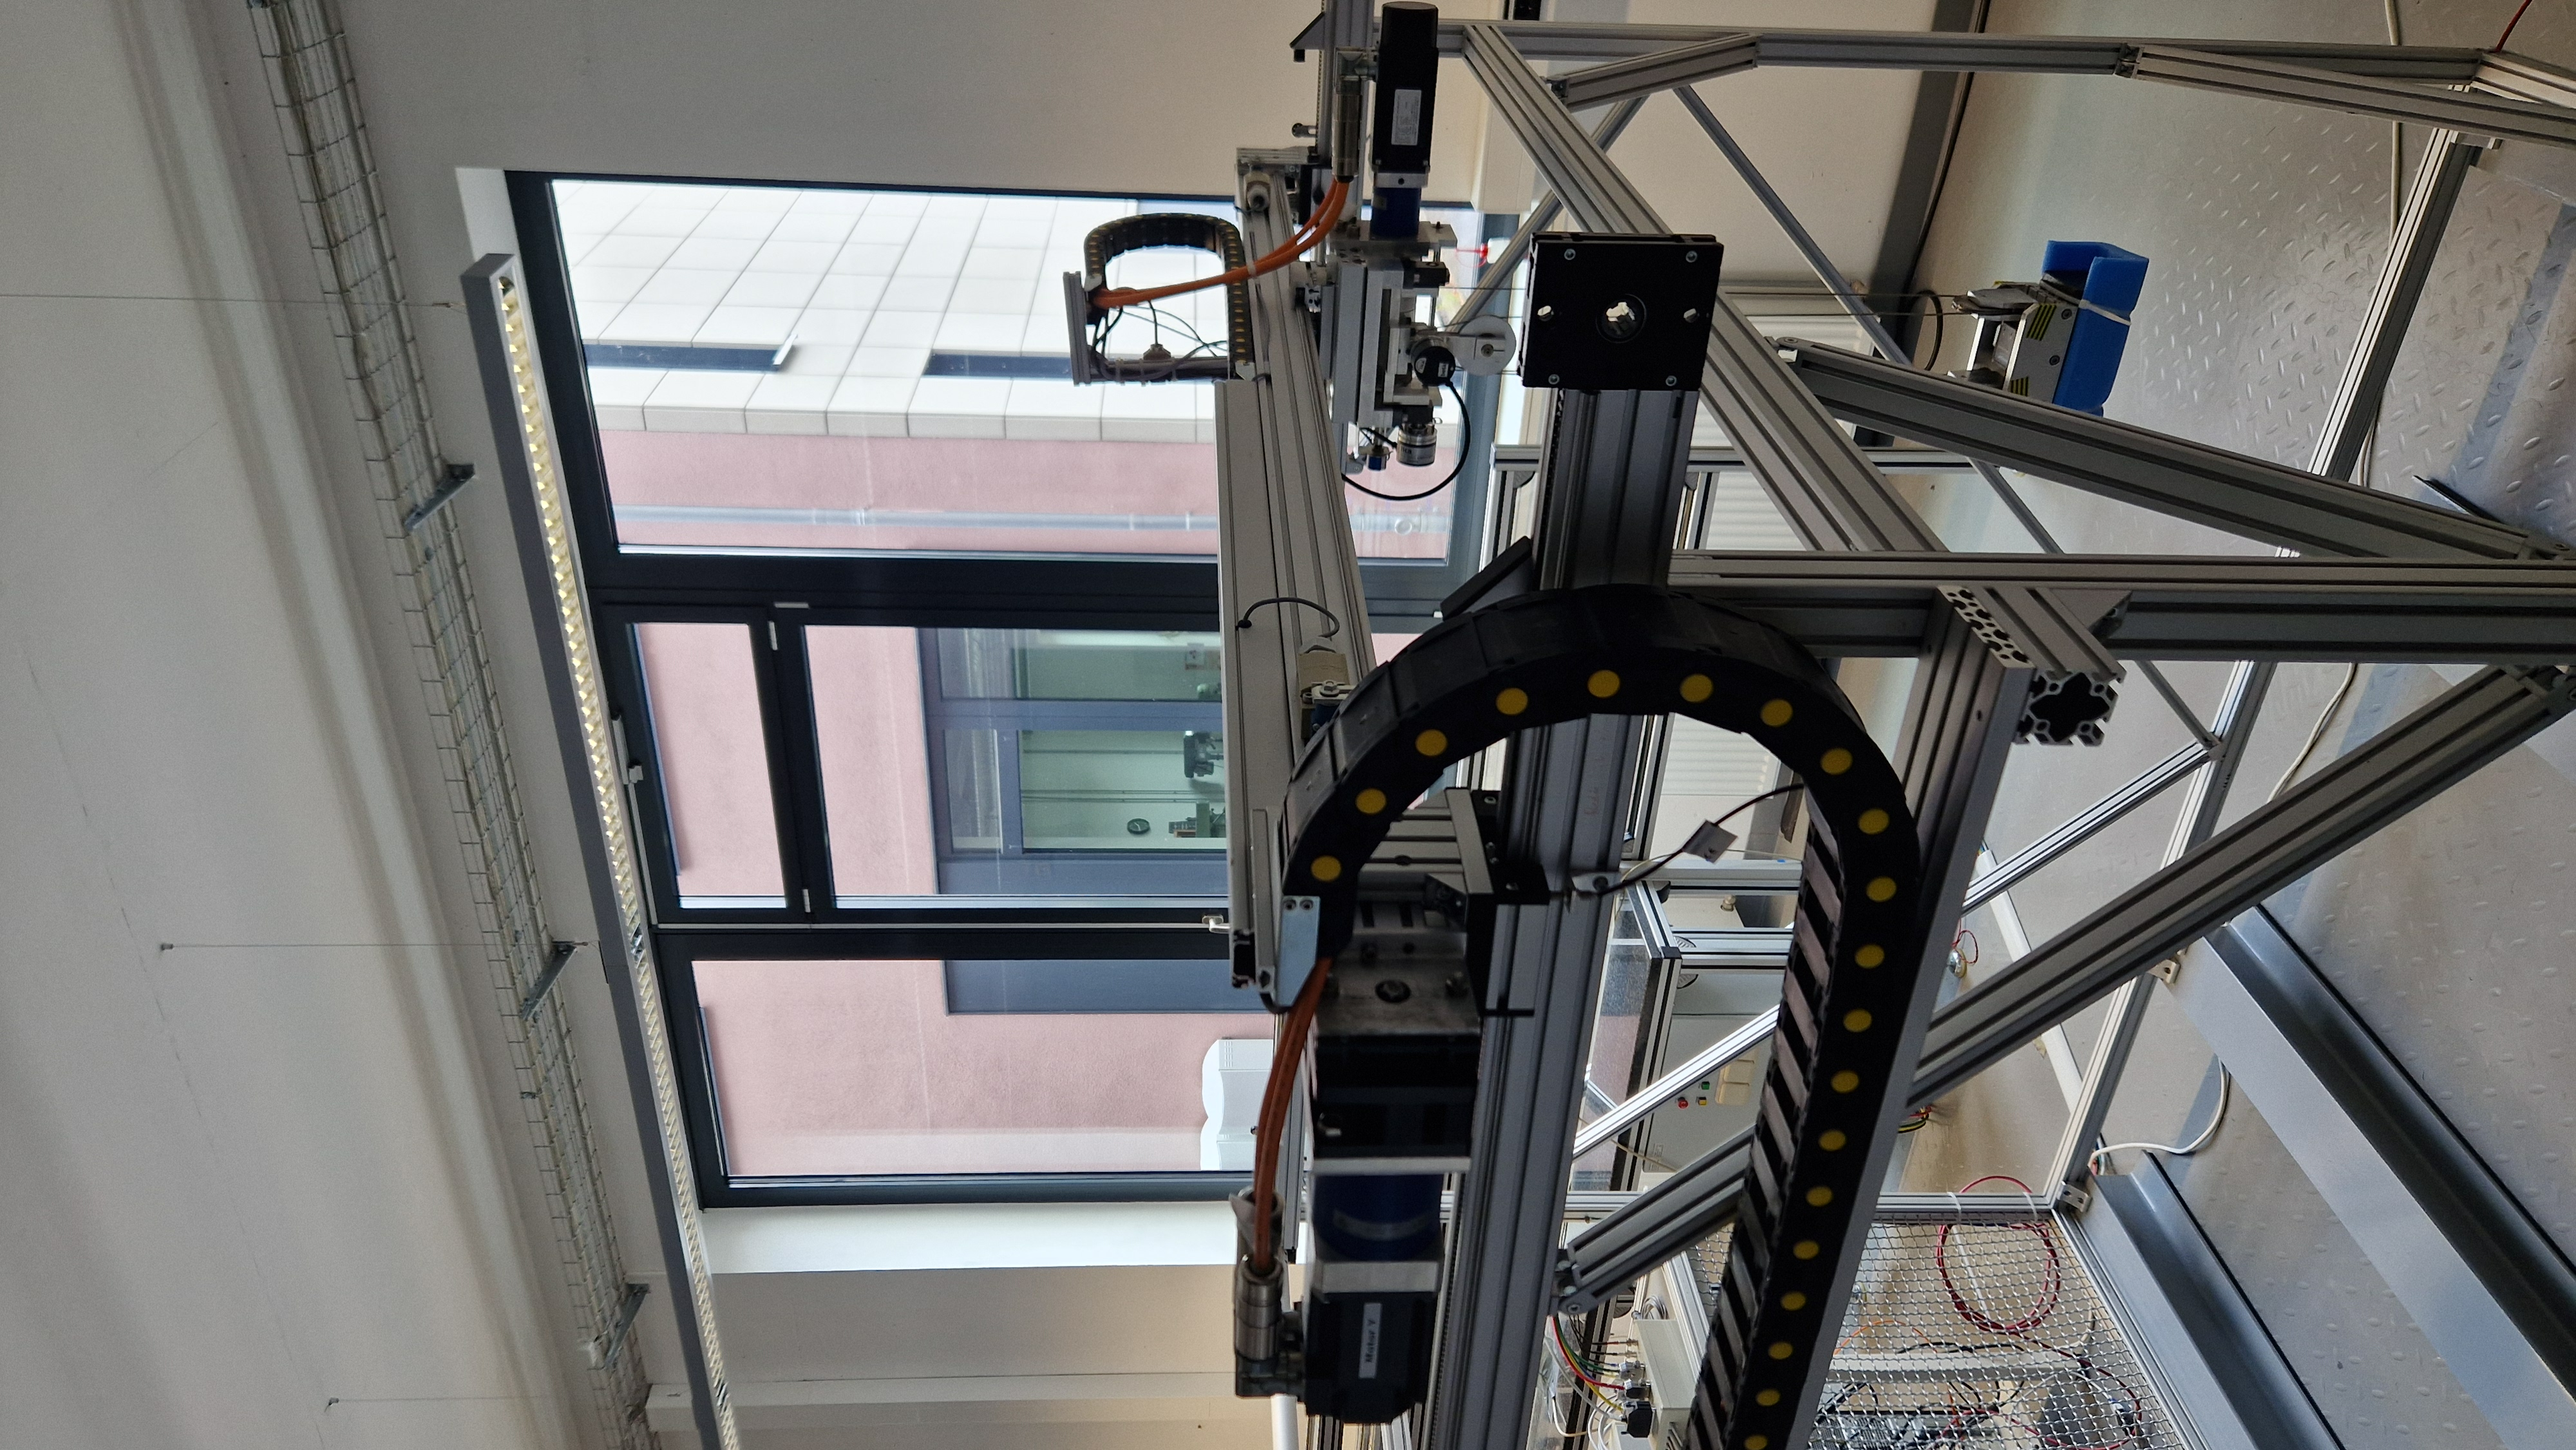
\includegraphics[width=\linewidth]{imgs/Simulation/Ymot.jpg}}
        \captionof{figure}{Zoom on Y motor}
    \end{column}
\end{columns}
\end{frame}

%_______________________________________________________________________%
\begin{frame}{Results}   
\end{frame}

\section{Conclusion}
\begin{frame}{Conclusion}
The main points to remember about Model Following Control (MFC) are:
\begin{itemize}
\item This control strategy can be applied to a wide range of real-world systems with input-to-state stable dynamics.
\item The design proposed by \cite{Tietze2023CruiseControl} provides a simple implementation compared to other techniques, which are less direct.
\item MFC can mitigate the peaking phenomenon, providing the advantages of High-Gain control without its drawbacks.
\item Perturbations can be easily counteracted by tuning \(\epsilon\), provided their bounds are known.
\end{itemize}
\end{frame}


\section{References}
\begin{frame}[allowframebreaks]{References}
    \bibliographystyle{plain}
    \bibliography{biblio.bib}
\end{frame}

\begin{frame}
\begin{center}
    Thank you! \\
    \email
\end{center}
\end{frame}

\end{document}

